\documentclass{article}
\usepackage{lmodern} % Fix the font size warnings
\usepackage{fancyhdr} % Required for custom headers
\usepackage{lastpage} % Required to determine the last page for the footer
\usepackage{extramarks} % Required for headers and footers
\usepackage{graphicx} % Required to insert images
\usepackage{xfrac} % Nice fractions
\usepackage{amsmath}
\usepackage{wrapfig}
\usepackage{blindtext}

\usepackage{multicol}

% Margins
\topmargin=-0.5in
\evensidemargin=0in
\oddsidemargin=-0.5in
\textwidth=7.5in
\textheight=9.0in
\headsep=0.25in 

% paragraphs
\usepackage{parskip}

\pagestyle{fancy}

\rhead{Desserts and sweets}
\lhead{\textbf{Oatmeal Cookies}}
\chead{}
\title{Oatmeal Cookies}

\begin{document}
I started with the ``classic'' recipe from the top of the Quaker Oats box. You know,
the one that \emph{everyone} uses? Well, I was never really a fan because those
cookies always came out flat and boring. Sometimes they'd be so flat it was like
eating a very flat thing. Anyway, after a lot of experimentation (well, three or
four batches), I came up with this recipe instead.

This recipe makes about 30 cookies.

\bigskip

\textbf{Ingredients}

\begin{multicols}{2}
      \begin{itemize}
            \item \sfrac{1}{2} cup (1 stick) plus 6 tablespoons butter, cold
            \item \sfrac{3}{4} cup packed dark brown sugar
            \item \sfrac{1}{2} cup granulated sugar
            \item 2 large eggs
            \item 1\sfrac{1}{2} teaspoons vanilla
            \item 1\sfrac{3}{4} cups, plus 2 tablespoons flour
            \item 1 teaspoon baking soda
            \item 2 teaspoons ground cinnamon
            \item \sfrac{1}{2} teaspoon salt
            \item 3\sfrac{1}{4} cups Quaker Oats
            \item (optional) 1 cup craisins or raisins
      \end{itemize}
\end{multicols}

\bigskip

\textbf{Directions}

\begin{enumerate}
      \item Adjust an over rack to the middle position and heat the oven to 350 degrees. Line a large baking sheet
            with parchment paper.
      \item Whisk the flour, baking soda, cinnamon, oats, and salt in a medium bowl and set aside.
      \item Cut the butter into tablespoon-sized pieces and beat on medium with the sugars until light and fluffy
            (about three minutes).
      \item Reduce speed to medium and add the eggs and vanilla. Increase speed to medium-high and beat until
            light and fluffy (the mixture will appear to double in size).
      \item Add the dry ingredients one cup at a time until fully incorporated. Scrap the sides of the
            bowl and mix at least one more time.
      \item Use a \#30 cookie dough scoop (the medium one) to form balls of dough.
            Place 2 inches apart on the parchment-lined baking sheets and bake for 9 minutes until just starting
            to turn medium brown. The cookies will still look slightly undercooked.
      \item Cool the cookies for 5 minutes on the baking sheet then move to a wire rack. Avoid the rush of people.
\end{enumerate}


\begin{wrapfigure}{L}{0.3\textwidth}
      \begin{center}
            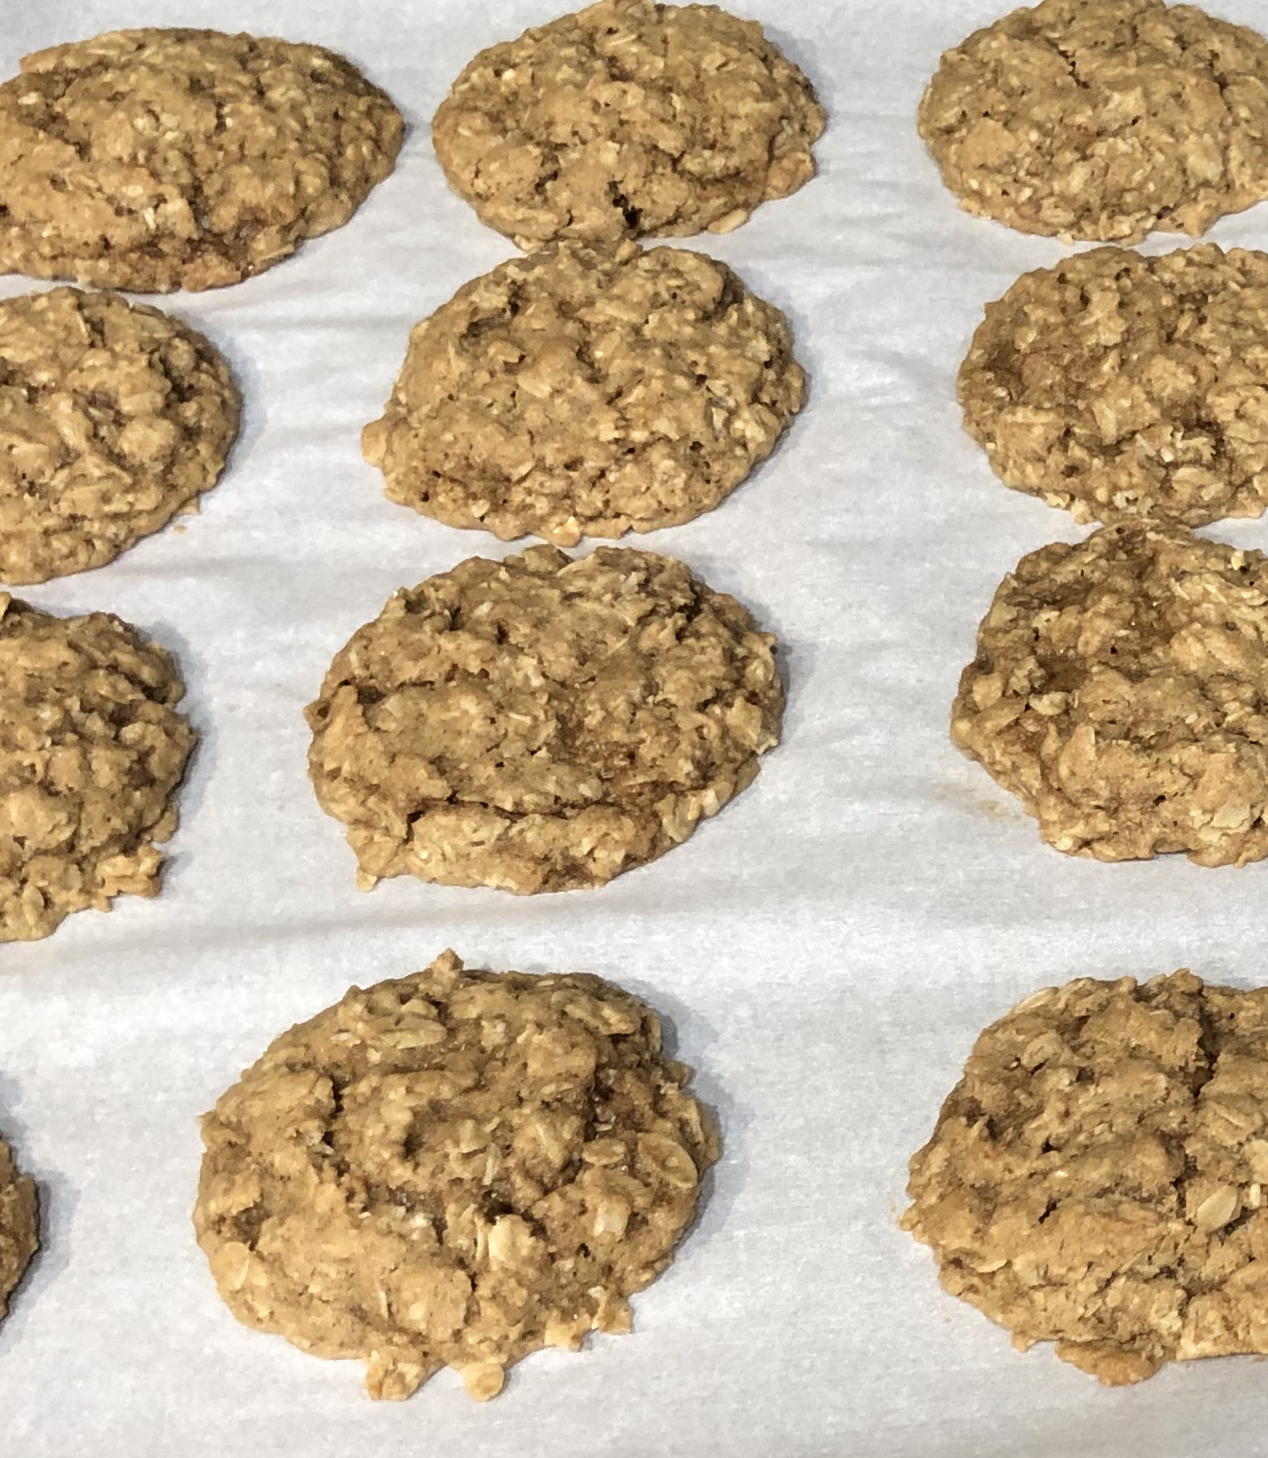
\includegraphics[width=0.25\textwidth]{oatmeal-cookies.png}
      \end{center}
\end{wrapfigure}

\bigskip

\textbf{Notes}

After making these Bill, Min's dad, mentioned that he'd made oatmeal cookies in the past using
Grand Marnier. That made me wonder if adding some grated orange peel would be good. Turns out that
I had one of these that happened to be sitting very close to a Sumo orange and the flavor
combination was \emph{nice}. So, I'm tempted to do this in my next batch.

\end{document}
